\documentclass[xcolor=table]{beamer}
\mode<presentation>
\usetheme{CambridgeUS}
\usepackage[english, russian]{babel}
\usepackage[utf8]{inputenc}
\usepackage[T2A]{fontenc}
\usepackage{sansmathaccent}
\usepackage{alltt}
\usepackage[table]{xcolor}
%\linespread{0.8}
\usepackage{minted}
\usepackage{setspace}

\usepackage{verbatim}
\usepackage{alltt}

\pdfmapfile{+sansmathaccent.map}
\title[Межпроцессное взаимодействие]{Обзор методов межпроцессного взаимодействия в Linux}
\author{Наумов Д.А., доц. каф. КТ}
\date[13.11.2020] {Операционные системы и системное программное обеспечение, 2020}

\begin{document}

%ТИТУЛЬНЫЙ СЛАЙД
\begin{frame}
  \titlepage
\end{frame}
  
%СОДЕРЖАНИЕ ЛЕКЦИИ
\begin{frame}
  \frametitle{Содержание лекции}
  \tableofcontents  
\end{frame}

\section{Обзор методов межпроцессного взаимодействия в Linux}

\subsection{Общие сведения о межпроцессном взаимодействии в Linux}

\begin{frame}
	В основе межпроцессного взаимодействия (IPC, InterProcess Communication) лежит обмен данными между работающими процессами. 

	Межпроцессное взаимодействие в \textit{Linux} можно классифицировать по трем критериям:
	\begin{itemize}
		\item По широте охвата взаимодействие бывает \textbf{локальным} и \textbf{удаленным}. Локальное взаимодействие подразделяется на \textbf{родственное} и \textbf{неродственное}.
		\item По направлению передачи данных межпроцессное взаимодействие бывает \textbf{однонаправленным} и \textbf{двунаправленным}.
		\item По характеру доступа взаимодействие бывает \textbf{открытым} и \textbf{закрытым}.
	\end{itemize}
	\begin{block}{Закрытое взаимодействие}
		осуществляется только между двумя процессами.
	\end{block}
	\begin{block}{Открытое взаимодействие}
		другой процесс может присоединиться к обмену данными.
	\end{block}
\end{frame}

\begin{frame}
	\begin{block}{Локальное взаимодействие}
		отвечает за обмен данными между процессами, которые работают в одной Linux-системе. Если обмен данными осуществляется между родительским и дочерним процессами, то такое взаимодействие называется 	\textit{родственным}.
	\end{block}
	\begin{block}{Удаленное взаимодействие}
		это обмен данными между двумя процессами, которые работают в разных системах. 
	\end{block}
	\begin{block}{Однонаправленное межпроцессное взаимодействие}
		характеризуется тем, что один процесс является отправителем данных, другой --- приемником этих данных.
	\end{block}
	\begin{block}{Двунаправленное взаимодействие}
	позволяет процессам общаться на равных, но в этом случае процессы должны <<договориться>> об очередности и синхронизации приема и передачи информации.
	\end{block}
\end{frame}

\begin{frame}
	Существование различных способов межпроцессного взаимодействия обусловлено тем, что при их реализации возникают две проблемы:
	\begin{enumerate}
		\item \textit{Проблема синхронизации}. Процессы работают независимо друг от друга, в ходе обмена данными между процессами должна учитываться эта <<независимость>>.
		\item \textit{Проблема безопасности}. 
		\begin{itemize}
			\item Если один процесс направляет данные другому процессу, то возникает опасность того, что потенциальный злоумышленник может перехватить эти данные. 
			\item Проблема усложняется еще и тем, что злоумышленник может "подсунуть" процессу-приемнику собственные данные, если последние не защищены. 
			\item Чем шире зона охвата межпроцессного взаимодействия, тем более уязвимым (с точки зрения безопасности) оно является.
		\end{itemize}
	\end{enumerate}
\end{frame}

\subsection{Локальные методы межпроцессного взаимодействия}

\begin{frame}{Локальные методы межпроцессного взаимодействия}
	Простейший способ межпроцессного взаимодействия:
	\begin{itemize}
		\item локальное 
		\item родственное 
		\item двунаправленное 
		\item закрытое 
\end{itemize}
	взаимодействие родителя и потомка.

	\medskip
	Родительский процесс может передавать дочернему некоторые данные посредством аргументов через одну из функций семейства \textbf{exec()}. 
	
	\medskip	
	В свою очередь дочерний процесс при нормальном завершении сообщает родителю свой код возврата.
\end{frame}

\begin{frame}[fragile]{Пример: kinsfolk-child1.c}
	\linespread{0.8}
	\begin{minted}{c}
#include <stdio.h>
#include <stdlib.h>
int main (int argc, char ** argv)
{
	int year;
	if (argc < 2) {
		fprintf (stderr, "child: too few arguments\n");
		return 2;
	}
	year = atoi (argv[1]);
	if (year <= 0)
		return 2;
	if ( ((year%4 == 0) && (year%100 != 0)) ||
			(year%400 == 0) )
		return 1;
	else
		return 0;	
	return 0;
}	
	\end{minted}
\end{frame}

\begin{frame}[fragile]{Пример: kinsfolk-parent1.c}
	\linespread{0.8}
	\begin{minted}{c}
#include <stdio.h>
#include <unistd.h>
#include <sys/types.h>
#include <wait.h>
int main (int argc, char ** argv)
{
  pid_t cpid;
  int status;	
  if (argc < 2) {
    fprintf (stderr, "Too few arguments\n");
    return 1;
  }	
  cpid = fork();
  if (!cpid) {
    execl ("./kinsfolk-child1", "Child", argv[1], NULL);
    fprintf (stderr, "execl() error\n");
    return 1;
  }
	\end{minted}
\end{frame}

\begin{frame}[fragile]{Пример: kinsfolk-parent1.c}
	\linespread{0.8}
	\begin{minted}{c}
  waitpid (cpid, &status, 0);
  if (WIFEXITED (status)) {
    if (WEXITSTATUS (status) == 1)
      printf ("%s: leap year\n", argv[1]);
    else if (WEXITSTATUS (status) == 0)
      printf ("%s: not leap year\n", argv[1]);
    else {
      fprintf (stderr, "error: unexpected "
               "return code\n");
      return 1;
    }
  }
  return 0;
}
	\end{minted}
\end{frame}

\begin{frame}[fragile]{Пример: kinsfolk-child1.c}
\begin{alltt}
\$ gcc -o kinsfolk-child1 kinsfolk-child1.c
\$ ./kinsfolk-child1 2007
\$ echo \$?
0

\$ ./kinsfolk-child1 2008
\$ echo \$?
1

\$ ./kinsfolk-child1 2300
\$ echo \$?
0

\$ ./kinsfolk-child1 2400
\$ echo \$?
1
\end{alltt}
\end{frame}

\begin{frame}[fragile]{Пример: kinsfolk-parent.c}
\begin{alltt}
\$ gcc -o kinsfolk-parent1 kinsfolk-parent1.c

\$ ./kinsfolk-parent1 2000
2000: leap year

\$ ./kinsfolk-parent1 2007
2007: not leap year
\end{alltt}
\end{frame}

\subsection{Удаленное межпроцессное взаимодействие}

\begin{frame}{Удаленное межпроцессное взаимодействие}
	\begin{block}{Сокет}
		комплексное понятие, которое условно можно назвать <<точкой соединения процессов>>
	\end{block}
	\begin{itemize}
		\item Unix-сокеты для локального взаимодействия процессов;
		\item Интернет-сокеты для удаленного взаимодействия процессов.
\end{itemize}
	В программах сокеты фигурируют в виде файловых дескрипторов, над которыми (во многих случаях) можно осуществлять обычные операции чтения-записи (read(), write() и т. д.). 
	\begin{itemize}
		\item При взаимодействии посредством сокетов процессы рассматриваются по схеме <<клиент — сервер>>.
		\item Процесс-сервер устанавливает <<правила общения>> и предлагает всем желающим межпроцессное взаимодействие. 
	\end{itemize}
\end{frame}

\section{Сигналы}

\begin{frame}{Понятие сигнала}
	\begin{block}{Cигнал}
		сообщение, которое один процесс-отправитель посылает другому процессу или самому себе.
	\end{block}
	\begin{itemize}
		\item В распоряжении процессов находится стандартный набор сигналов, заранее определенных ядром \textit{Linux}.
		\item Каждый сигнал имеет свой уникальный номер, а также символическую константу, соответствующую этому номеру. 
	\end{itemize}
	Процесс-получатель может отреагировать на сигнал одним из следующих трех способов:
	\begin{itemize}
		\item \textbf{Принятие сигнала}. Обычно это приводит к немедленному завершению процесса.
		\item \textbf{Игнорирование сигнала}. Процесс может установить для себя политику игнорирования определенных сигналов. 
		\item \textbf{Перехватывание и обработка сигнала}. Процесс может задать собственное поведение в отношении конкретного сигнала.
	\end{itemize}
\end{frame}

\begin{frame}[fragile]
	\begin{figure}[h]
		\centering
		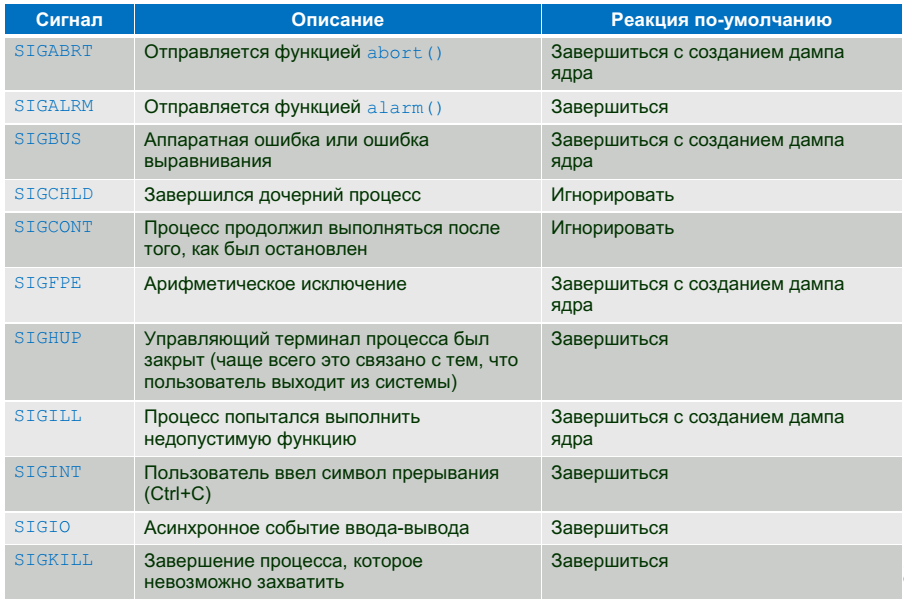
\includegraphics[scale=0.5]{images/signals.png}
	\end{figure}
\end{frame}

\begin{frame}[fragile]
	\begin{figure}[h]
		\centering
		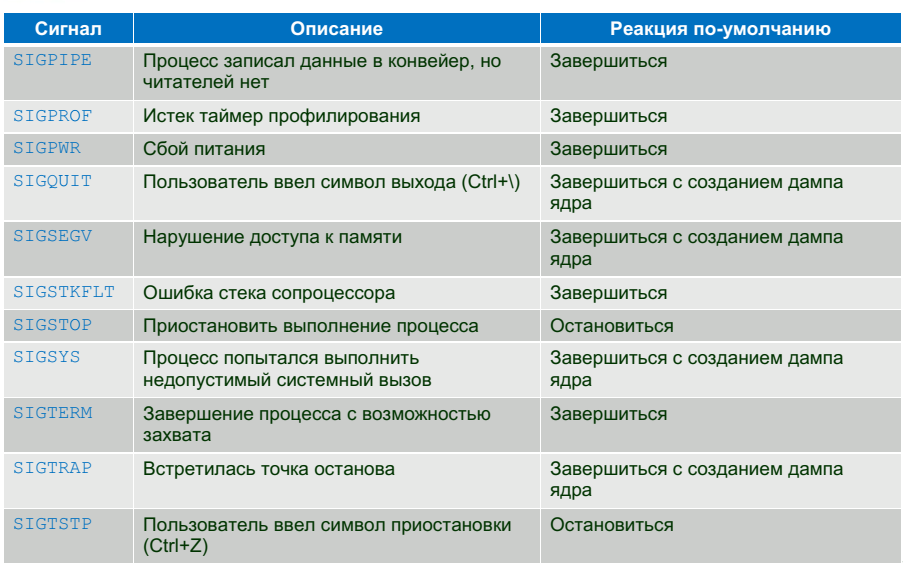
\includegraphics[scale=0.5]{images/signals-2.png}
	\end{figure}
\end{frame}

\begin{frame}[fragile]
	\begin{figure}[h]
		\centering
		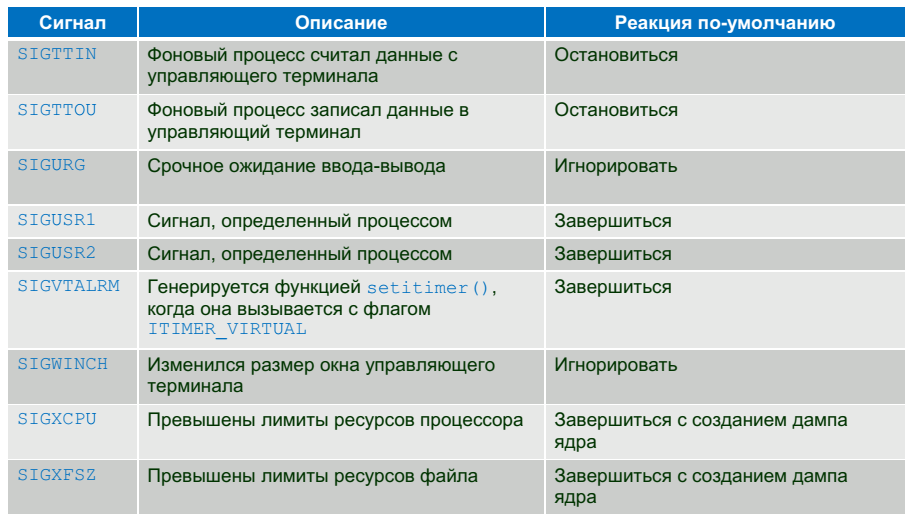
\includegraphics[scale=0.5]{images/signals-3.png}
	\end{figure}
\end{frame}

\begin{frame}[fragile]
\begin{alltt}
\$ kill -s SIGNAL PID
\end{alltt}
Здесь SIGNAL — это символическая константа посылаемого сигнала, PID — идентификатор процесса-получателя сигнала. 
\begin{alltt}
\$ yes > /dev/null &
[1] 5852
\$ ps
PID TTY TIME CMD
5481 pts/2 00:00:00 bash
5852 pts/2 00:00:04 yes
5853 pts/2 00:00:00 ps
\$ kill -s SIGINT 5852
\$ ps
PID TTY TIME CMD
5481 pts/2 00:00:00 bash
5854 pts/2 00:00:00 ps
[1]+ Interrupt yes >/dev/null
\end{alltt}
\end{frame}

\begin{frame}[fragile]{Отправка сигнала kill()}
	Для отправки сигнала предусмотрен системный вызов \textit{kill()}, который объявлен в заголовочном файле \textit{signal.h} следующим образом:
	\begin{minted}{c}
int kill (pid_t PID, int SIGNAL);
	\end{minted}
	Этот системный вызов посылает процессу с идентификатором \textit{PID} сигнал \textit{SIGNAL}.

	\medskip
	Возвращаемое значение --- 0 (при успешном завершении) или -1 (в случае ошибки).

	\medskip
	Если в аргументе \textit{PID} системного вызова \textit{kill()} указать текущий идентификатор, то процесс пошлет сигнал сам себе. 
\end{frame}

\begin{frame}[fragile]{Пример: kill1.c}
	\linespread{0.8}
	\begin{minted}{c}
#include <signal.h>
#include <stdio.h>
#include <stdlib.h>

int main (int argc, char ** argv)
{
  pid_t dpid;
  if (argc < 2) {
    fprintf (stderr, "Too few arguments\n");
    return 1;
  }
  dpid = atoi (argv[1]);
  
  if (kill (dpid, SIGKILL) == -1) {
    fprintf (stderr, "Cannot send signal\n");
    return 1;
  }	
  return 0;
}
	\end{minted}
\end{frame}

\begin{frame}[fragile]{Пример: kill2.c}
	\linespread{0.8}
	\begin{minted}{c}
#include <signal.h>
#include <stdio.h>
#include <stdlib.h>

int main (void)
{
  pid_t dpid = getpid ();

  if (kill (dpid, SIGABRT) == -1) {
    fprintf (stderr, "Cannot send signal\n");
    return 1;
  }
  return 0;
}
	\end{minted}
\end{frame}

\begin{frame}[fragile]{Обработка сигнала sigaction()}
	Системный вызов sigaction() позволяет задавать поведение процесса по отношению к конкретным сигналам:
	\begin{minted}{c}
int sigaction (int SIGNAL, const struct sigaction * ACTION, 
    struct sigaction * OLDACTION);
	\end{minted}
	Данный системный вызов устанавливает политику реагирования процесса на сигнал SIGNAL. Политика определяется указателем ACTION на структуру типа sigaction. При удачном завершении функции по адресу OLDACTION заносится прежняя политика в отношении сигнала. 

~

	Структура sigaction содержит различные поля:
	\begin{itemize}
		\item sa\_handler — адрес функции-обработчика сигнала; 
		\item sa\_flags — набор флагов. Для простой обработки сигнала достаточно обнулить это поле;
		\item sa\_mask — маска сигналов. Список сигналов, которые будут заблокированы во время работы функции-обработчика. 
	\end{itemize}
\end{frame}

\begin{frame}[fragile]{Пример: sigaction1.c}
	\linespread{0.8}
	\begin{minted}{c}
#include <signal.h>
#include <stdio.h>

void sig_handler (int snum){
	fprintf (stderr, "signal...\n");
}

int main (void)
{
	struct sigaction act;
	sigemptyset (&act.sa_mask);
	act.sa_handler = &sig_handler;
	act.sa_flags = 0;
	if (sigaction (SIGINT, &act, NULL) == -1) {
		fprintf (stderr, "sigaction() error\n");
		return 1;
	}
	while (1);
	return 0;
}
	\end{minted}
\end{frame}

\begin{frame}[fragile]{Пример sigaction1.c}
	Системный вызов sigaction() позволяет задавать поведение процесса по отношению к конкретным сигналам:
\begin{alltt}
\$ gcc -o sigaction1 sigaction1.c
\$ ./sigaction1
signal...
signal...
signal...
signal...
\end{alltt}
	Обратите внимание, что каждый раз при нажатии клавиш Ctrl+C процесс реагирует мгновенно. 

~

	При использовании сигналов всегда следует помнить, что на момент получения сигнала программа может выполнять что-то важное.
	\begin{alltt}
\$ ps -e | grep sigaction1
4883 pts/1 00:44:27 sigaction1
\$ kill 4883
	\end{alltt}
\end{frame}

\begin{frame}[fragile]{Сигналы и многозадачность}
	Если во время выполнения функции-обработчика процесс получает еще один сигнал, программа может начать вести себя неадекватно.
\begin{itemize}
	\item включить в обработчик сигнала минимальное число инструкций. Лучше, если это будет одна инструкция, которая просто устанавливает флаг, регистрирующий получение сигнала. 
	\item программа может при необходимости проверять значение этого флага и реагировать соответствующим образом.
	\item применяется специальный тип данных sig\_atomic\_t - обычное целое число, но ядро Linux гарантирует, что математические операции над таким числом являются атомарными и не могут быть прерваны.
\end{itemize}
Пример 1: sigaction2.c

Пример 2: kinsfolk-child2.c, kinsfolk-parent2.c
\end{frame}

\begin{frame}[fragile]{Пример: sigaction2.c}
	\linespread{0.8}
	\begin{minted}{c}
sig_atomic_t sig_occured = 0;
void sig_handler (int snum){
	sig_occured = 1;
}
int main (void)
{
  struct sigaction act;
  sigemptyset (&act.sa_mask);
  act.sa_handler = &sig_handler;
  act.sa_flags = 0;
  if (sigaction (SIGINT, &act, NULL) == -1) {
    fprintf (stderr, "sigaction() error\n");
    return 1;
  }
  while (1) {
    if (sig_occured) {
      fprintf (stderr, "signal...\n"); sig_occured = 0;
    }
  }	
  return 0; }
	\end{minted}
\end{frame}

\begin{frame}[fragile]{Пример: kinsfolk-child2.c}
	\linespread{0.8}
	\begin{minted}{c}
#include <stdio.h>
#include <stdlib.h>
#include <signal.h>
#include <unistd.h>
int main (int argc, char ** argv)
{
  int year;
  if (argc < 2) {
    fprintf (stderr, "child: too few arguments\n");
    return 2;
  }
  year = atoi (argv[1]);
  if (year <= 0)
    return 2;
  if (((year%4==0)&&(year%100!=0))||(year%400==0))
    kill (getppid (), SIGUSR1);
  else
    kill (getppid (), SIGUSR2);
  return 0;
}
	\end{minted}
\end{frame}

\begin{frame}[fragile]{Пример: kinsfolk-parent2.c}
	\linespread{0.8}
	\begin{minted}{c}
#include <stdio.h>
#include <unistd.h>
#include <sys/types.h>
#include <wait.h>
#include <signal.h>

/* 0 - no signal, 1 - SIGUSR1, 2 - SIGUSR2 */
sig_atomic_t sig_status = 0;

void handle_usr1 (int s_num)
{
  sig_status = 1;
}

void handle_usr2 (int s_num)
{
  sig_status = 2;
}
	\end{minted}
\end{frame}

\begin{frame}[fragile]{Пример: kinsfolk-parent2.c}
	\linespread{0.8}
	\begin{minted}{c}
int main (int argc, char ** argv)
{
  struct sigaction act_usr1, act_usr2;
  sigemptyset (&act_usr1.sa_mask);
  sigemptyset (&act_usr2.sa_mask);
  act_usr1.sa_flags = 0;
  act_usr2.sa_flags = 0;
  act_usr1.sa_handler = &handle_usr1;
  act_usr2.sa_handler = &handle_usr2;

  if (sigaction (SIGUSR1, &act_usr1, NULL) == -1) {
    fprintf (stderr, "sigaction (act_usr1) error\n");
    return 1;
  }
  if (sigaction (SIGUSR2, &act_usr2, NULL) == -1) {
    fprintf (stderr, "sigaction (act_usr2) error\n");
    return 1;
  }
  if (argc < 2) {
    fprintf (stderr, "Too few arguments\n");
    return 1;
  }	
	\end{minted}
\end{frame}

\begin{frame}[fragile]{Пример: kinsfolk-parent2.c}
	\linespread{0.8}
	\begin{minted}{c}
  if (!fork()) {
    execl ("./kinsfolk-child2", "Child", argv[1], NULL);
    fprintf (stderr, "execl() error\n");
    return 1;
  }
  while (1) {
    if (sig_status == 1) {
      printf ("%s: leap year\n", argv[1]);
      return 0;
    }
    if (sig_status == 2) {
      printf ("%s: not leap year\n", argv[1]);
      return 0;
    }
  }
  return 0;
}	
	\end{minted}
\end{frame}

\section{Использование общей памяти}

\begin{frame}[fragile]{Использование общей памяти}
	Реализация межпроцессного взаимодействия посредством совместно используемой памяти:
	\begin{enumerate}
		\item один из процессов выделяет некоторый объем памяти, который называется сегментом. К общему сегменту памяти привязаны два числа:
		\begin{itemize}
			\item Идентификатор сегмента — служит для доступа к сегменту внутри процесса.
			\item Ключ сегмента — идентифицирует сегмент для других процессов. Ключ может быть выделен автоматически во время создания сегмента. Процессы могут также заранее договориться о применении определенного статического ключа.
		\end{itemize}
		\item после выделения совместно используемого сегмента другие процессы могут задействовать его. 
\end{enumerate}
\end{frame}

\begin{frame}[fragile]{Выделение общей памяти}
	Выделение общей памяти осуществляется при помощи системного вызова \textbf{shmget()}, который объявлен в заголовочном файле \textit{sys/shm.h} следующим образом:
	\begin{minted}{c}
int shmget (key_t KEY, size_t SIZE, int FLAGS);
	\end{minted}
	\begin{itemize}
		\item KEY — это ключ сегмента. Если взаимодействующие программы не договорились заранее о применении статического ключа, то в данном поле можно указать константу IPC\_PRIVATE, которая инициирует динамическое выделение ключа.
		\item SIZE — размер сегмента. Здесь следует учитывать, что данный аргумент является запрашиваемым числом байтов для сегмента. Реально выделенное число байтов может отличаться от SIZE.
		\item Аргумент FLAGS определяет права доступа к совместно используемому сегменту, а также дополнительные флаги.
	\end{itemize}
\end{frame}

\begin{frame}[fragile]{Активизация совместного доступа}
	Процесс может получить доступ к созданному сегменту двумя способами:
	\begin{itemize}
		\item Использовать идентификатор сегмента, полученный от другого процесса.
		\item Вызвать \textit{shmget()}, применяя для этого заранее известный ключ.
	\end{itemize}
	Для работы с общим сегментом памяти нужно, чтобы каждый из взаимодействующих процессов обратился к системному вызову \textit{shmat()}:
	\begin{minted}{c}
void * shmat (int ID, void * ADDRESS, int FLAGS);
	\end{minted}
	Данный системный вызов возвращает адрес совместно используемого сегмента памяти. 
	\begin{itemize}
		\item ID — это идентификатор сегмента. 
		\item ADDRESS - адрес, по которому будет доступен общий сегмент памяти. 
		\item FLAGS - дополнительные флаги.
	\end{itemize}
\end{frame}

\begin{frame}[fragile]{Отключение совместного доступа}
	Системный вызов \textbf{shmdt()} вызывается в каждом процессе после того, как тот закончил работу с общей памятью. 
	\begin{minted}{c}
int shmdt (void * ADDRESS);
	\end{minted}
	\begin{itemize}
		\item ADDRESS — это адрес совместно используемой памяти, который возвращает shmat() при подключении сегмента.
	\end{itemize}
	Системный вызов \textbf{shmctl()} позволяет осуществлять различные операции над общим сегментом памяти.
	\begin{minted}{c}
int shmctl (int ID, int COMMAND, struct shmid_ds * DESC);
	\end{minted}
	\begin{itemize}
		\item ID — это идентификатор сегмента. 
		\item COMMAND — команда, которую требуется выполнить в отношении сегмента общей памяти с идентификатором ID. Часто употребляются две команды: IPC\_STAT (получить данные о сегменте) и IPC\_RMID (удалить сегмент).
		\item DESC — указатель на структуру, в которую (для команды IPC\_STAT) заносятся данные о сегменте. 
	\end{itemize}
\end{frame}

\begin{frame}[fragile]{Пример}
	\textbf{shm1-owner.c}
	\begin{itemize}
		\item Программа создает общий сегмент с использованием "динамического ключа" (IPC\_PRIVATE). 
		\item После успешного создания и подключения сегмента программа выводит на экран его идентификатор, заносит в сегмент данные и останавливается до тех пор, пока пользователь не нажмет клавишу Enter. 
		\item Эта задержка позволяет другому процессу подключить общий сегмент памяти и прочитать оттуда данные.
\end{itemize}
	\textbf{shm1-user.c}
	\begin{itemize}
		\item Поскольку процессы "не договорились" заранее о выделении общего ключа для сегмента памяти, то единственным адекватным способом взаимодействия будет непосредственная передача программе-клиенту идентификатора сегмента через аргумент.
	\end{itemize}
\end{frame}

\begin{frame}[fragile]{Пример}
	В первом окне запускаем процесс-сервер:
	\begin{alltt}
\$ gcc -o shm1-owner shm1-owner.c
\$ ./shm1-owner
ID: 31391750
Press <Enter> to exit...
	\end{alltt}
	Теперь, не нажимая клавиши <Enter>, переходим в другое терминальное окно и запускаем процесс-клиент:
	\begin{alltt}
\$ gcc -o shm1-user shm1-user.c
\$ ./shm1-user 31391750
Message: Hello World!
	\end{alltt}
\end{frame}

\begin{frame}[fragile]{Пример}
	Наберите в клиентском окне команду \textbf{ipcs -m}. Эта команда выводит на экран список совместно используемых сегментов памяти с их ключами и идентификаторами. 
\begin{alltt}
\$ ipcs -m
------ Shared Memory Segments --------
key shmid owner perms bytes nattch status
0x00005d8b 13565953 root 777 316 1
0x00000000 13795330 nn 600 393216 2 dest
0x00000000 13828099 nn 600 393216 2 dest
0x00000000 29589508 nn 666 112320 1 dest
0x00000000 14811141 nn 777 393216 2 dest
0x00000000 31391750 nn 600 4096 1
\end{alltt}
\end{frame}

\begin{frame}[fragile]{Пример}
Теперь нажмите клавишу Enter в исходном терминале и вызовите \textbf{ipcs -m} еще раз:
\begin{alltt}
\$ ipcs -m
------ Shared Memory Segments --------
key shmid owner perms bytes nattch status
0x00005d8b 13565953 root 777 316 1
0x00000000 13795330 nn 600 393216 2 dest
0x00000000 13828099 nn 600 393216 2 dest
0x00000000 29589508 nn 666 112320 1 dest
0x00000000 14811141 nn 777 393216 2 dest
\end{alltt}
\end{frame}

\section{Использование общих файлов}

\begin{frame}[fragile]{Использование общих файлов}
	Системный вызов mmap() позволяет частично или целиком отображать в оперативной памяти содержимое файла.
	\begin{minted}{c}
void * mmap (void * ADDRESS, size_t LEN, int PROT,
             int FLAGS, int FD, off_t OFFSET);
	\end{minted}
	\begin{itemize}
		\item ADDRESS - адрес, по которому будет отображаться файл. Если указать здесь NULL, то адрес будет выбран автоматически.
		\item LEN - размер отображаемой области.
		\item PROT - уровень защиты отображаемой области. Этот аргумент может состоять из побитовой дизъюнкции флагов PROT\_READ (чтение), PROT\_WRITE (запись) и PROT\_EXEC (выполнение).
		\item FLAGS - при реализации межпроцессного взаимодействия этот аргумент обычно принимает значение MAP\_SHARED.
		\item FD — дескриптор открытого файла, который будет отображаться в памяти.
		\item OFFSET — смещение, от которого будет отображаться файл.
	\end{itemize}
\end{frame}

\begin{frame}[fragile]{Использование общих файлов}
	Системный вызов \textbf{munmap()} освобождает отображаемую область памяти.
	\begin{minted}{c}
int munmap (void * ADDRESS, size_t LEN);
	\end{minted}
	\begin{itemize}
		\item ADDRESS - буфер отображаемой памяти, который будет освобожден.
		\item LEN - размер отображаемой области.
	\end{itemize}
	Пример: mmap1.c
	\begin{alltt}
\$ gcc -o mmap1 mmap1.c
\$ echo "" > myfile
\$ echo -n LINUX >> myfile
\$ ./mmap1 myfile
\$ cat myfile
XUNIL
	\end{alltt}
\end{frame}

\begin{frame}[fragile]{Пример: mmap1.c}
	\linespread{0.8}
	\begin{minted}{c}
#include <stdio.h>
#include <string.h>
#include <sys/mman.h>
#include <fcntl.h>
#include <unistd.h>

#define FLENGTH 256

void reverse (char * buf, int size)
{
	int i;
	char ch;
	for (i = 0; i < (size/2); i++)
	{
		ch = buf[i];
		buf[i] = buf[size-i-1];
		buf[size-i-1] = ch;
	}
}
	\end{minted}
\end{frame}

\begin{frame}[fragile]{Пример: mmap1.c}
	\linespread{0.8}
	\begin{minted}{c}
int main (int argc, char ** argv)
{
	int fd;
	char * buf;
	if (argc < 2) {
		fprintf (stderr, "Too few arguments\n");
		return 1;
	}

	fd = open (argv[1], O_RDWR);
	if (fd == -1) {
		fprintf (stderr, "Cannot open file (%s)\n",
				argv[1]);
		return 1;
	}
	\end{minted}
\end{frame}

\begin{frame}[fragile]{Пример: mmap1.c}
	\linespread{0.8}
	\begin{minted}{c}

	buf = mmap (0, FLENGTH, PROT_READ | PROT_WRITE,
			MAP_SHARED, fd, 0);
	if (buf == MAP_FAILED) {
		fprintf (stderr, "mmap() error\n");
		return 1;
	}

	close (fd);
	reverse (buf, strlen (buf));

	munmap (buf, FLENGTH);
	return 0;
}	
	\end{minted}
\end{frame}

\begin{frame}[fragile]{Использование общих файлов}
	\begin{itemize}
		\item Данные файла, отображаемые в памяти, на самом деле существуют отдельно от самого файла. 
		\item Если отображаемая область изменяется, то сброс данных файла на носитель осуществляется только при вызове \textbf{munmap()}. 
		\item Однако использование отображаемых в памяти файлов при реализации межпроцессного взаимодействия зачастую требует осуществить сброс данных на носитель (синхронизацию) без отключения отображаемой области.
\end{itemize}
	Это позволяет делать системный вызов \textbf{msync()}
\begin{minted}{c}
int msync (void * ADDRESS, size_t LEN, int FLAGS);
\end{minted}
	\begin{itemize}
	\item ADDRESS - буфер отображаемой памяти, который будет освобожден.
	\item LEN - размер отображаемой области.
	\end{itemize}
\end{frame}

\section{Каналы}

\begin{frame}
  \frametitle{Содержание лекции}
  \tableofcontents[current]
\end{frame}

\begin{frame}[fragile]{Создание канала: pipe()}
	\begin{itemize}
		\item Каналы осуществляют в Linux родственное локальное межпроцессное взаимодействие. 
		\item Интерфейс канала представляет собой два связанных файловых дескриптора, один из которых предназначен для записи данных, другой — для чтения. 
		\item Возможность родственного межпроцессного взаимодействия через канал обусловлена тем, что дочерние процессы наследуют от родителей открытые файловые дескрипторы.
	\end{itemize}
	Для создания канала служит системный вызов pipe():
	\begin{minted}{c}
int pipe (int PFDS[2]);
	\end{minted}
	При успешном завершении системного вызова pipe() в текущем процессе появляется канал
	\begin{itemize}
		\item запись в который осуществляется через дескриптор PFDS[0], 
		\item чтение - через PFDS[1]. 
	\end{itemize}
\end{frame}

\begin{frame}[fragile]{Создание канала: pipe()}
	\begin{itemize}
		\item Данные, передаваемые через канал, практически не нуждаются в разделении доступа. 
		\item Канал автоматически блокирует читающий или пишущий процесс, когда это необходимо. 
		\item Если читающий процесс запрашивает больше данных, чем есть в настоящий момент в канале, то процесс блокируется до тех пор, пока в канале не появятся новые данные.
	\end{itemize}
	Закрытие <<концов>> канала осуществляется при помощи системного вызова close()
	\begin{minted}{c}
int close (int fd);
	\end{minted}
	\begin{itemize}
	\item закрытие дескриптора происходит только тогда, когда все процессы, разделяющие этот дескриптор, вызовут close().
	\end{itemize}
\end{frame}

\begin{frame}[fragile]{Создание канала: pipe()}
Пример: pipe1-parent.c, pipe1-src.c, pipe1-dst.c
\begin{alltt}
\$ gcc -o pipe1-parent pipe1-parent.c
\$ gcc -o pipe1-src pipe1-src.c
\$ gcc -o pipe1-dst pipe1-dst.c
\$ ./pipe1-parent
Wait please.....
Hello World
\end{alltt}
\end{frame}

\begin{frame}[fragile]{Перенаправление ввода-вывода: dup2()}
Системный вызов dup2() позволяет перенаправлять ввод-вывод. 
\begin{alltt}
int dup2 (int FD1, int FD2);
\end{alltt}
Системный вызов dup2() перенаправляет ввод-вывод с дескриптора FD2 на дескриптор FD1. 

Пример: dup01.c. Программа выводит сообщение "Hello World!" посредством функции printf().
Но системный вызов dup2() перенаправил стандартный вывод (дескриптор 1) в файл. Поэтому после работы программы текст "Hello World!" окажется не на экране терминала, а в файле myfile:
\begin{alltt}
\$ gcc -o dup01 dup01.c
\$ ./dup01
\$ cat myfile
Hello World!
\end{alltt}
\end{frame}

\begin{frame}[fragile]{Перенаправление ввода-вывода: dup2()}
Пример: dup02.c. 

Программа осуществляет перенаправление стандартного ввода: при попытке прочитать что-нибудь из стандартного ввода программа выведет на экран содержимое файла myfile:
\begin{alltt}
\$ gcc -o dup02 dup02.c
\$ echo "Hello World" > myfile
\$ ./dup02
Hello World
\end{alltt}
\end{frame}

\begin{frame}[fragile]{Перенаправление ввода-вывода: dup2()}
Аргументами dup2() могут быть дескрипторы канала. Это позволяет налаживать взаимодействие любых процессов, которые используют в своей работе консольный ввод-вывод. 

Пример: pipe2.c. 
\begin{itemize}
\item программа принимает два аргумента: имя каталога и произвольную строку. 
\item программа вызывает команду ls для первого аргумента и grep -i для второго. 
\item при этом стандартный вывод ls связывается со стандартным вводом grep. 
\item В итоге на экран выводятся все элементы указанного каталога, в которых содержится строка (без учета регистра символов) из второго аргумента.
\end{itemize}
\begin{alltt}
\$ gcc -o pipe2 pipe2.c
\$ ./pipe2 / bin
bin
sbin
Hello World
\end{alltt}
\end{frame}

\section{Именованные каналы FIFO}

\begin{frame}[fragile]{Именованные каналы FIFO}
\begin{itemize}
\item Именованные каналы FIFO работают аналогично обычным. 
\item Особенность FIFO в том, что они представлены файлами специального типа и "видны" в файловой системе. 
\item Работа с этими файлами осуществляется обычным образом при помощи системных вызовов open(), close(), read(), write() и т. д. Это, позволяет использовать их вместо обычных файлов. 
\item Через FIFO могут взаимодействовать процессы, не являющиеся ближайшими родственниками.
\end{itemize}

Именованные каналы создаются командой mkfifo и удаляются командой rm:
\begin{alltt}
\$ mkfifo myfifo
\$ ls -l myfifo
prw-r--r-- 1 nn nn 0 2011-05-11 09:57 myfifo
\$ rm myfifo
\end{alltt}
В расширенном выводе программы ls каналы FIFO обозначаются символом p (от англ. pipe). 
\end{frame}

\begin{frame}[fragile]{Именованные каналы FIFO}
Работать с FIFO можно даже без написания специальных программ. Проведем небольшой эксперимент:
\begin{alltt}
\$ mkfifo myfifo
\$ cat myfifo
\end{alltt}
Поскольку канал FIFO пуст, то программа cat оказалась заблокированной. Для снятия блокировки откроем новое окно терминала и введем следующую команду:
\begin{alltt}
\$ echo "Hello World" > myfifo
\end{alltt}
В первом окне будет написано сообщение "Hello World" и программа cat завершится.
\end{frame}

\begin{frame}[fragile]{Именованные каналы FIFO}
Для создания именованных каналов FIFO предусмотрен системный вызов mkfifo()
\begin{alltt}
int mkfifo (const char * FILENAME, mode_t MODE);
\end{alltt}
\begin{itemize}
\item FILENAME - это имя файла, 
\item MODE - права доступа. 
\end{itemize}

Создание именованного канала FIFO, имя которого передается через аргумент:
\begin{alltt}
if (mkfifo (argv[1], 0640) == -1) \{
  fprintf (stderr, "Can't make fifo");
  return 1;
\}
\end{alltt}
\end{frame}

\begin{frame}[fragile]
Каналы FIFO функционируют аналогично обычным каналам.
\begin{itemize}
\item Если канал опустел, то читающий процесс блокируется до тех пор, пока не будет прочитано заданное количество данных или пишущий процесс не вызовет close().
\item И наоборот, пишущий процесс "засыпает", если данные не успевают считываться из FIFO.
\end{itemize}
Пример: fifo2-server.c, fifo2-client.c 

Если запустить "сервер", то он создаст FIFO и "замрет" в ожидании поступления данных:
\begin{alltt}
\$ gcc -o fifo2-server fifo2-server.c
\$ ./fifo2-server
\end{alltt}
Запустим теперь в другом терминальном окне клиентскую программу:
\begin{alltt}
\$ gcc -o fifo2-client fifo2-client.c
\$ ./fifo2-client Hello
\end{alltt}
Серверный процесс тут же "проснется", выведет сообщение "Hello" и завершится.
\end{frame}

\end{document} 
